BERT(Bidirectional Encoder Representations from Transformers)とは,Google が2018年に発表した自然言語処理モデルである\cite{bert}.Recurent Neural Network などを使わずに Attention機構のみを用いた Transformer \cite{transformer} と呼ばれるモデルがある.Transformer が 文脈を単一方向しか考慮しないのに対して,双方向考慮するように改良したのが BERT である.BERT の特徴として,事前学習モデルであることが挙げられる.従来のニューラルネットワークを用いた自然言語処理モデルは,言語理解や感情推定など特定のタスクのみに対応しており,タスクに応じた出力を行う.しかし,事前学習モデルである BERT は既存のタスク実行モデルに付け加えるだけで,そのモデルの性能を向上させることが可能である.
\par
BERT を付け加える際には,入出力をタスクに合わせたものに置き換えて追加学習する Fine-Tuning という手法が用いられる.そのようなモデルの中での BERT は,入力文の埋め込み表現を得るために用いられる.自然言語処理における埋め込みとは,文や単語,文字など自然言語の構成要素に対して,何らかの空間におけるベクトルを与えることであり,ベクトルには文や単語の特徴量が格納される.図\ref{fig:bert_fine}のように,BERTは2つの文章を入力として,単語単位に分割する.分割したものをトークンと呼ぶ.また,入力した文の初めに“[CLS]”,2つの文章の末尾に“[SEP]”という特殊なトークンを挿入する.そして,BERTは文章ペア全体の埋め込み表現とトークンレベルの埋め込み表現を抽出する.BERTに付け加えたタスク実行モデルは,これら埋め込み表現を用いて各タスクに合わせた出力を学習していく.また,BERT 自体もタスクに合うように埋め込み表現を更新していく.
\par
  
\begin{figure}[tbh]
  \centering
  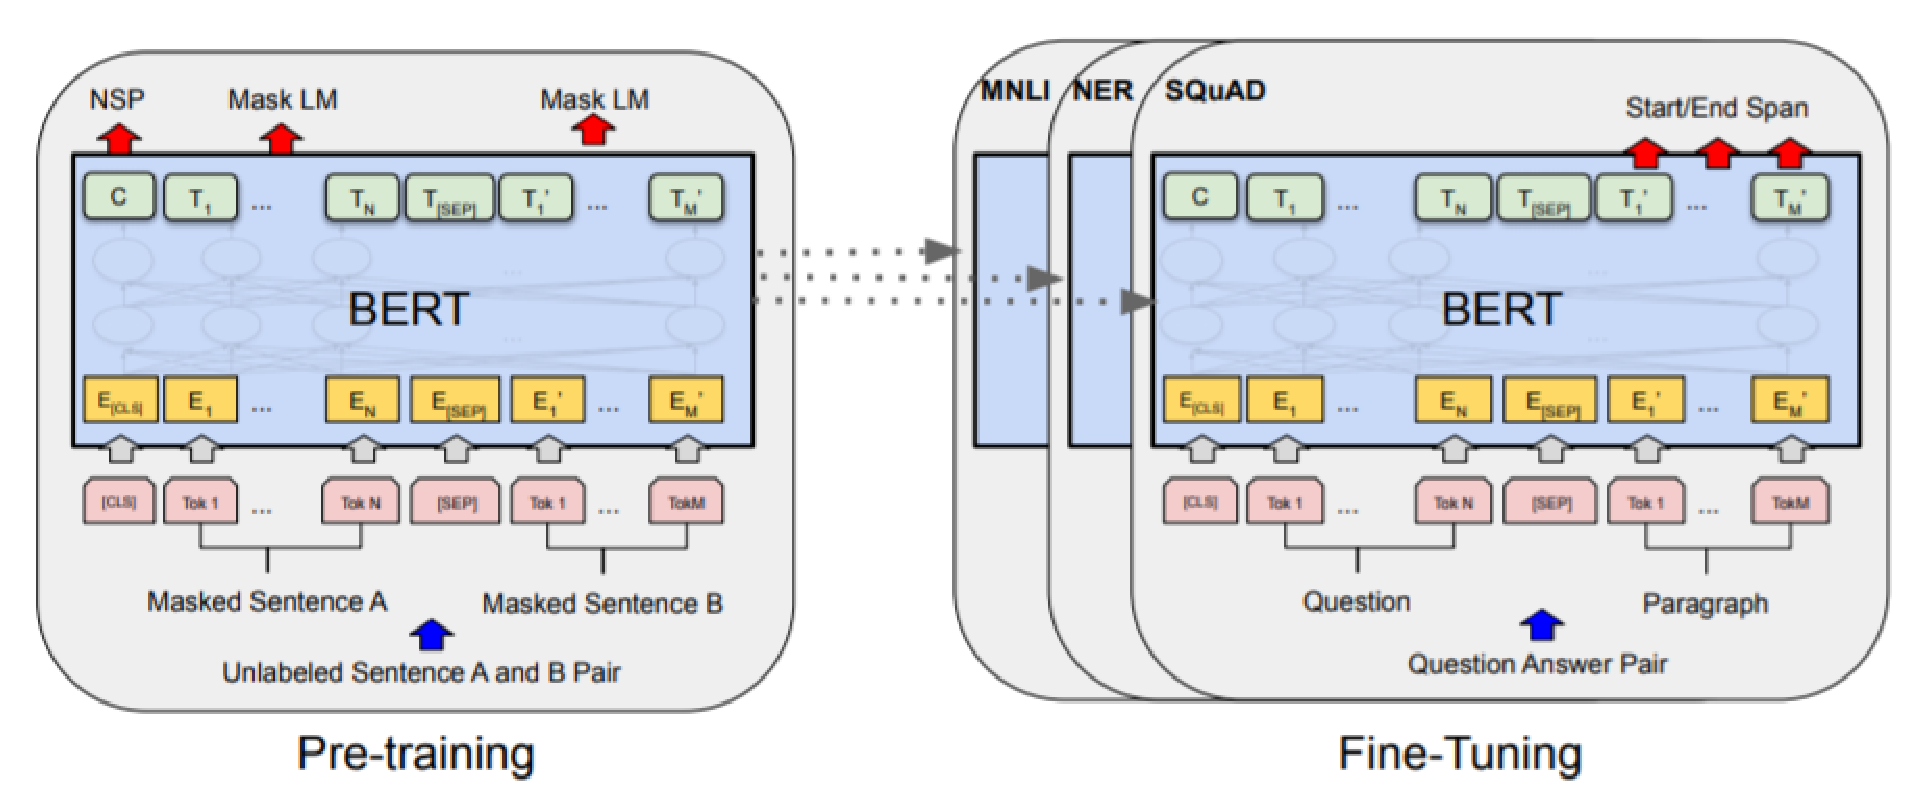
\includegraphics[width=15cm]{chapter3/bert_fine.eps}
  \caption{Fine-Tuningの例\cite{bert}}
  \label{fig:bert_fine}
\end{figure}

BERT は汎用性の高さが評価され注目を浴びている.加えて,少ないデータで追加学習を行うだけで動作するため,自然言語処理分野の長年の課題であったデータ不足を解決する.自然言語処理分野でデータが不足していた原因は,データ収集やラベルの付与に多大なコストと時間がかかることが挙げられる.しかし,BERT の事前学習では Wikipedia や BooksCorpus などから得た大量のラベル未付与のデータを用いて,前後の文脈を加味したトークンの埋め込み表現や2つの文章の関係性を事前に学習する.そのため,少量のラベル付きデータで追加学習を行うだけでタスクの実行が可能になる.ゆえに,本研究でも BERT による対話状態追跡モデルをベースラインとして用いる.